\chapter{\IfLanguageName{dutch}{Stand van zaken}{State of the art}}%
\label{ch:stand-van-zaken}

% Tip: Begin elk hoofdstuk met een paragraaf inleiding die beschrijft hoe
% dit hoofdstuk past binnen het geheel van de bachelorproef. Geef in het
% bijzonder aan wat de link is met het vorige en volgende hoofdstuk.

% Pas na deze inleidende paragraaf komt de eerste sectiehoofding.
\section{Educatieve Technologie in de 21e Eeuw}
In de 21e eeuw is technologie niet meer weg te denken uit de samenleving. Echter is dit ook zo in scholen. Wanneer er wordt ingezoomd op de leeromgeving waar leerlingen en studenten zich bevinden, zijn er veel veranderingen opgetreden. ``Klaslokalen over de hele wereld worden technologisch steeds geavanceerder. Een groeiende trend is dat scholen elke leerling een persoonlijke laptop of tablet ter beschikking stellen, zowel voor gebruik in de klas als thuis.'' \textcite{HALL2021101957} Dit alles is in een versneld tempo geëvolueerd na de COVID-pandemie. Waardoor scholen ook in een versneld tempo moesten schakelen om deze vereisten op te zetten in hun gebouwen, denk maar aan meer stopcontacten, beter internet, betere informatica apparatuur en middelen voor arme gezinnen.\newline
Vervolgens moesten de scholen hun leerpakketten ook aanpassen zodat leerlingen meer met de computer konden werken tijdens de lessen. Hierdoor waren leerkrachten in staat tot overschakeling van zelfstandiger onderwijs. Anderzijds toont onderzoek aan dat leerlingen sneller afgeleid zijn bij het gebruik van laptops en tablets in de les. \textcite{deng2020laptops} Met betrekking tot het bekijken van E-commerce websites en het gebruiken van sociale media. Hierdoor was er dus nood aan verscheidene methoden of technologieën die in staat zijn de leerlingen toch bij de les te houden en controle uit te voeren tijdens de lessen. Deze technologieën worden ook wel Classroom management software (CMS) genoemd.

\section{Sociale Media versus E-commerce}
In de moderne samenleving is het gebruik van sociale media en E-commerce niet meer weg te denken. Hoewel beiden online platformen zijn, wordt er nadrukkelijk onderscheid gemaakt in functionaliteiten, doelstellingen en impact op gebruikers van beiden. Om goed te begrijpen waarom deze twee online platformen educatief worden ingezet in de lessen is het noodzakelijk om diepgaand inzicht te krijgen in de definitie en het onderscheid tussen deze twee. \newline
\subsection{Wat is Sociale media}
``Sociale media is een verzamelnaam voor websites en applicaties die zich richten op communicatie, community-based input, interactie, het delen van content en samenwerking.`` \autocite{Lutkevich_Wigmore_2021}
Wanneer sociale media in kaart wordt gebracht kennen de meeste personen verscheidene opties, zoals Facebook, Instagram, X en Linkedin. Natuurlijk bestaan er nog meerdere sociale media platforms maar dit zijn slechts voorbeelden. Het primaire doel van sociale media is zorgen voor communicatie, interactie en het geven van meningen tussen verschillende personen en groepen over de hele wereld. \newline

\subsection{Wat is E-commerce}
Een minder bekend begrip is E-Commerce platformen, wat op twee verschillende manieren kan worden gedefinieerd. 
\begin{itemize}
    \item  ``Een E-commerce platform is dus een softwareapplicatie die helpt bij het bouwen van een eigen online winkel. De software zorgt ervoor dat je als webwinkel eenvoudig online je verkoopactiviteiten kunt beheren. Elk platform heeft zijn eigen voor-en nadelen en de functionaliteiten verschillen per aanbieder.''\autocite{Elbertse_2021} 
    \item ``Het kopen en verkopen van goederen en diensten over het internet.''\autocite{e-commerce2024}
\end{itemize}
Voorbeelden van E-commerce platformen zijn Amazon, Zalando, Alibaba en Shein. Het hoofddoel van deze platformen is het faciliteren van transacties tussen kopers en verkopers, waarbij de focus ligt op het maken van omzet en winst door commerciële activiteiten. \newline

\subsubsection{Onderscheid tussen Sociale media en E-commerce}
Het onderscheid tussen sociale media en E-commerce is essentieel om hun bijdrage te leveren in educatieve doeleinden. Terwijl sociale media zich voornamelijk richt op het communiceren en interactie tussen personen, bieden E-commerce platformen zich op mogelijkheden tot aanschaffen van goederen en diensten in het onderwijs. Met name het aanschaffen van boeken, cursussen en leermateriaal. Door deze verschillen naast elkaar te leggen kan het onderwijs strategieën uitrollen voor de implementatie van beiden in een educatieve omgeving.\newline
\subsection{Integratie van Sociale Media en E-commerce tijdens de lessen}
Eerder werd door \textcite{Purwanto2023} onderzoek gedaan naar het gebruik van sociale media tijdens de lessen. Het onderzocht toonde aan dat sociale media in vele gevallen ook positief kan zijn in het onderwijs, zowel voor leerlingen als leerkrachten. Het gebruik ervan kan dienen als direct communicatiemiddel tussen leerkracht en student, waar sociale media wordt ingezet om aankondigingen en updates te plaatsen om zo discussies in vermijden. 
Vervolgens kan de studentenbetrokkenheid verhoogd worden dankzij sociale media tools. Naast de stimulatie van leerlingen zorgen deze platforms ook voor actieve deelname aan het vormgeven van de eigen leerervaring. Hierdoor kunnen studenten zich comfortabel uiten, samenwerken en waardevolle leermiddelen delen en raadplegen, onafhankelijk van tijd en plaats. \newline
Tot slot wordt er in de studie nog een laatste aspect besproken, namelijk sociale media als samenwerkingsplatform. Hierbij bevordert de samenwerking tussen leerlingen, leerkrachten en andere betrokkenen door kennis uit te wisselen. Zo kunnen samenwerkingstools zoals 'Google Docs' makkelijker worden gedeeld en kan ieder zijn steentje bijdragen door gebruik te maken van gedeelde inhoud. Op deze manier wordt de samenwerking tussen leerlingen verbeterd. \newline
De voordelen van sociale media leggen de basis bij het gebruik van E-commerce platforms tijdens de lessen, waarbij gevaarlijke en foute verkoopsites worden aangekaart om leerlingen te waarschuwen voor frauduleuze websites. Wat resulteert in oplettende studenten die zich ervan bewust zijn dat niet elke reclame betrouwbaar is. Hierdoor gaan jongeren meer nadenken vooraleer ze een bestelling plaatsen op een onbekende website. \autocite{Purwanto2023} \autocite{onlinefraude}

\section{Wat is open-source software}
In een hedendaagse digitale wereld, waar hardware en software een onmisbare rol spelen in het dagelijkse leven, is het concept van open-source software van groot belang. Om de context en resultaten van deze bachelorproef te begrijpen en te waarderen, is het essentieel om het begrip open-source uitgebreid uit te leggen.\newline

Over het algemeen is er geweten dat scholen weinig budget hebben te besteden bovenop vaste kosten. Met die reden wordt IT-infrastructuur vaak verwaarloost, waardoor nood aan open-source programma's en toestellen een must zijn. Open-source software is de software waarbij broncode volledig toegankelijk en gratis beschikbaar is voor iedereen. Dit betekend dat iedereen de code mag bekijken, aanpassen, kopiëren en opnieuw verspreiden zonder enige beperkingen of licentiekosten. Daarentegen bij gesloten source software is de broncode geheim en mogen alleen de ontwikkelaars of eigenaars aanpassingen op de software uitvoeren. \newline

Er zijn tal van voordelen aan het gebruik van open-source software. Naast de verschillende voordelen die hierboven zijn opgesomd, is open source vaak ook gratis. Hierdoor is het voor consumenten zoals scholen, overheidsinstanties en andere organisaties met een beperkt budget heel aantrekkelijk om deze vorm van software te gebruiken.

Vervolgens is open-source software vrij aanpasbaar, zo kan de software worden afgestemd aan de behoeften van de gebruikers. Dit alles omdat de broncode beschikbaar is, kunnen ontwikkelaars de code aanpassen naar hun eigen wensen. Dit maakt open-source nog aantrekkelijker voor andere bedrijven en instanties met enige informatica kennis. 

Tot slot is open source software beter beveiligd omdat beveiligingsexperten betere controles kunnen uitvoeren door middel van de vrij beschikbare broncode. Dit omdat er sneller kan worden op gereageerd en geanticipeerd wanneer fouter of zwakke plekken opduiken. \autocite{opensource}

\section{Wat is Classroom management software}
\label{classroom management software}
Classroom management software (CMS) stelt leerkrachten in staat om de apparaten van leerlingen te bekijken, controleren en te beheren. Ook biedt deze software leerkrachten een overzicht van alle deelnemende leerlingen hun scherm en beidt het de mogelijkheid om verdere controle over deze computers over te nemen. \autocite{brioso2017classroom}
Populaire voorbeelden hiervan zijn: Veyon, Moodle en Mythware Classroom management software, natuurlijk zijn er nog tal van voorbeelden. Maar als er gefilterd wordt op open-source komen deze drie er als beste uit.  
Kenmerkend aan deze software is de verscheidene functies die gebruikers hiermee kunnen verwezenlijken
\begin{itemize}
    \item Beheer alle lessen vanaf de startpagina: door gebruik te maken van de startpagina kunnen lessen centraal beheerd worden. Bij de meeste classroom management software is het mogelijk om hierop alle computers van de desbetreffende virtuele klas waar te nemen.
    \item Creëren van virtuele groepen: door gebruik te maken van virtuele groepen, worden de desbetreffende computers gekoppeld aan een virtuele klas. Hierdoor kan de leerkracht beter overzicht bewaren en klas per klas gaan bekijken.
    \item Stuur expresberichten naar de schermen van leerlingen hun apparaten: door gebruik te maken van een berichtomgeving kunnen leerkrachten communiceren via de computer om zo de leerlingen individueel aan te spreken zonder andere klasgenoten te storen tijdens de les.
    \item Push links naar een leerling of de hele klas: Deel bronnen, websites of aanvullend materiaal door links te pushen naar individuele groepen of naar de gehele klas. Hierdoor kunnen leerlingen sneller en efficiënter de nodige informatie bekomen, die worden gebruikt in de lessen.
    \item Ontvang updates over de status van studenten: door het gebruik van real-time updatestatussen is het handig om te weten waar een leerling zich bevindt in de opdracht. Zodoende krijgt de leerkracht inzicht in de activiteiten en prestaties, die de leerlingen op dat moment uitvoeren.
    \item Tel webregels in om specifieke websites te beperken: dit garandeert een veilige en gepaste online leeromgeving, waar leerlingen enkele de vooropgestelde websites kunnen bereiken die de leerkracht activeert en deactiveert. Hierdoor kunnen leerlingen bijvoorbeeld geen sociale media of E-commerce websites opzoeken. Wat resulteert in een grotere focus op de leerstof.
    \item Onderzoek de browsergeschiedenis van leerlingen: door gebruik te maken van inzicht in browsergeschiedenis is het mogelijk dat leerkrachten elke opzoekingsregel van de leerlingen kunnen waarnemen. Dit verhindert het ongepast gebruik van het internet en afleiding van de concentratie. 
    \item Bekijk schermen van de hele klas in één keer of zoom in op een afzonderlijk scherm: door monitoringsmethodes toe te passen is toezicht en directe ondersteuning van leerlingen mogelijk. Zodoende kan de leerkracht de leerlingen observeren tijdens individuele opdrachten of activiteiten.
    \item Registreer de activiteit op het scherm van een leerling: door middel van de opname modus bij vele classroom management software is het mogelijk dat de schermen van de leerlingen opgenomen worden. Dit kan handig zijn in het leerproces maar vooral tijdens het maken van online toetsen of taken is dit zeker geen overbodige optie. Eveneens biedt dit ook de kans tot persoonlijke feedback naar leerlingen toe.
\end{itemize}
De documentatie van \textcite{veyonhome} beschrijft de algemene functionaliteiten van Classroom management software die ook toepasbaar zijn bij andere tools. Dit omvat een duidelijk overzicht voor de gehele verzameling van Classroom management tools. 
Door gebruik te maken van deze software wordt er voor verscheidene scholen een oplossing geboden voor aandacht in de lessen, maar ook het flexibel beheren van rechten op het internet. 

\subsection{Beveiliging en privacy van Classroom management software}
\label{beveiliging en privacy CMS}
Doordat deze programma's verschillende schermen kunnen weergeven van elke leerling, is het uiteraard belangrijk dat deze programma's goed beveiligd worden. Ook moeten er duidelijke regels opgesteld worden voor de leerkrachten. Denk maar aan het gebruik van deze programma's buiten de school zelf. Tevens worden de virtuele klassen versleuteld zodat geen enkel persoon kan meekijken tijdens de les. Vooraleer leerkrachten toegang mogen verschaffen tot de controle van ieders scherm moeten de leerlingen het privacybeleid van de school goedkeuren. Wanneer ze dit niet goedkeuren mag de leerkracht geen gebruik maken van het programma bij de desbetreffende leerling. \autocite{privacy}

\section{Soorten Classroom management software}
Zoals in \ref{classroom management software} besproken, komen er drie open-source tools uit. Dit met als reden er sommige tools vroeger niet volledig open-source beschikbaar waren, maar nu zijn samengevoegd met een andere tools of niet relevant zijn voor deze casus. Voorbeelden hiervan zijn Impero, Classcraft en iTALC.
Hieronder worden de volgende drie classroom management software tools onder de loep genomen. 

\subsection{Veyon}
Veyon (Virtual Eye On Networks) is een open-source en robuuste software programma voor klasmanagement. Het biedt een breed assortiment aan functies zodat elke school zijn eigen omgeving kan creëren. Om verdere verwarring te voorkomen, wordt in deze software gesproken over een master-pc en een client-pc, waarbij de master-pc verwijst naar de computer van de leerkrachten en de client-pc naar de computer van de studenten. 

\subsubsection{Voordelen}
\begin{itemize}
    \item Gemakkelijke gebruiksomgeving: de gebruikersomgeving beschikt over een zeer flexibele en duidelijke interface. Wat voor leerkrachten met weinig informatica kennis makkelijk maakt om hiermee aan de slag te gaan. 
    \item Beperkte hard- en software vereisten: voor de client pc wordt er geen enkele speciale vereisten vooropgesteld. Desondanks er voor de master pc een vooropgestelde vereiste van minstens 2GB RAM geheugen en per client pc 20-30 MB beschikbaar is. Daarnaast wordt er een multi-core systeem van 2-4 CPU cores aangeraden.   
    \item Beschikbaar op Linux en Windows
    \item Automated/silent mode installatie: tijdens de installatie wordt er een volledig geautomatiseerde methode gehanteerd. Om die reden is het zeer makkelijk om grote hoeveelheden computer tegelijkertijd te installeren en configureren. 
    \item Veilig: door de aanwezigheid van authentication methodes wordt er zowel encryptie op de logingegevens toegepast als de beveiliging tussen de master pc en de client pc's. Deze 2 soorten authentication methodes zijn login authentication en key file authentication.
    \item Betrouwbaar: doordat Veyon al bestaat vanaf 2004 en voorkomt van het programma iTALC, is het betrouwbare software. Eveneens worden de updates nadrukkelijk bijgehouden zodat er steeds nieuwe versies beschikbaar zijn.
    \autocite{veyon} 
\end{itemize}
\subsubsection{Nadelen}
\begin{itemize}
    \item Internetconnectie vereist: wanneer deze uitvalt is het mogelijk dat het hele programma op elke computer zowel client als master volledig moet worden herstart. Met mogelijks tijdverlies als gevolg, bij het afnemen van belangrijke testen. 
    \item Betalende add-ons: Veyon beidt een aantal betalende add-ons die extra functionaliteiten en features aan het programma toevoegen zoals Internet acces control, chat, extra ID Connector, LDAP pro,  network discovery en screen recorder.
    \autocite{junghans-2023}
\end{itemize}

\subsection{Moodle}
Moodle is een open-source en krachtig software programma. Deze classroom manamegement software is ook gekend als leermanagement software. Wat ook betrekking heeft tot het creëren, beheren en bekijken van online lesmateriaal. 
\subsubsection{Voordelen}
\begin{itemize}
    \item Mogelijkheden: door de grote van de software en de vele features, is het mogelijk om een hele scholengroep te voorzien op dezelfde software
    \item Beschikbaarheid: doordat de software over de hele wereld bekent is, heeft het ook te maken met een grote hoeveelheid gebruikers. Hierdoor is de garantie op beschikbaarheid groot.
\end{itemize}
\subsubsection{Nadelen}
\begin{itemize} 
    \item Complexiteit: door de vele features van de software is het voor leerlingen en leerkrachten moeilijk om dit te leren. Ook betrekt deze software zich niet alleen tot classroom management wat een complexe gebruikersomgeving weergeeft. 
    \item Ingewikkelde installatie: door de vele mogelijkheden in de software, neemt de installatie meer tijd in beslag. Dit resulteert in een mindere aantrekkelijkheid naar kleinere schoolomgevingen zoals in deze casus.
    \item Benodigdheden: door de vele functionaliteiten van de software heeft het veel meer dan alleen maar een paar computers nodig. Er moet standaard een webserver, databaseserver en PHP geïnstalleerd zijn. 
    \autocite{moodle}
\end{itemize} 
\subsection{Mythware}
Mythware is een veelzijdige open-source software tool die niet alleen fungeert als classroom management software, echter biedt het ook andere functies aan om het onderwijsproces te verbeteren zoals evaluatie, beveiliging en volledige analyse over tablet gebruik. Deze casus beperkt zich alleen tot het beoordelen van de voor- en nadelen van de classroom management software wel kunnen de veelzijdige functies in het achterhoofd worden gehouden. Eveneens wordt er gesproken over de master pc en de client pc zoals bij Veyon.
\subsubsection{Voordelen}
\begin{itemize}
    \item Beschikbaar op Windows, Android, Ios, Mac OS en Linux
    \item Veelzijdige functies: naast het hoofddoel van deze casus biedt deze software ook andere functies aan. Enkele voorbeelden zijn het samenwerken tussen computers, smartphones en projectors of het geven van feedback op ontwerpen die leerlingen maakten op hun eigen apparaat maar ook network management en het opnemen van leerlingen hun apparaten.
    \item Gebruiksvriendelijk: de interface van zowel de master pc als de client pc zijn zeer gebruiksvriendelijk en makkelijk te leren. Hierdoor is complexiteit van het leerproces niet van toepassing. 
\end{itemize}
\subsubsection{Nadelen}
\begin{itemize} 
    \item Niet alle functies zijn voor alle besturingssystemen: het is niet mogelijk om met een Android of IOS apparaten blokkades op websites flexibel te beheren of toe te passen. Tevens zijn er andere features alleen mogelijk op Windows en Mac OS apparaten.
    \item Beperkt in talen: het is niet mogelijk om de taal van het programma in het Nederlands om te zetten. Wat het leerproces sterk kan beïnvloeden.
    \item Instapkosten bij het downloaden
    \autocite{mythware}
    \end{itemize}
\subsection{Conclusie}
Na grondig analyseren van verschillende open-source classroom management software mogelijkheden, waaronder Veyon, Moodle en Myhtware, lijkt Veyon de meest geschikte oplossing voor de proof of concept. Met zijn gebruiksvriendelijke interface, beperkte hard- en software vereisten en beschikbaarheid op Windows en Linux, biedt Veyon een ideale oplossing voor klaslokaalbeheer. Hoewel Mythware ook aantrekkelijke functies heeft, zoals veelzijdigheid en beschikbaarheid op meerdere besturingssystemen, kunnen beperkingen zoals het ontbreken van het Nederlands de gebruikservaring beïnvloeden. Anderzijds is Moodle ook heel krachtig maar door zijn hoge complexiteit van installatie en beheer, en hogere focus op leermanagement in plaats van classroom management beheer komt deze niet in aanmerking in deze casus. Concluderend biedt Veyon de beste combinatie van gebruiksgemak, betrouwbaarheid en effectieve functies voor het beheren en installeren van computers in scholen.

\section{Wat is een proxyserver}
Een andere manier voor dit te controleren is een proxy server. ``Een proxy (of proxyserver) is een computer die tussen een gebruiker en het internet in staat. De gebruiker van de proxy stuurt al zijn of haar internetverkeer naar de proxyserver. De server stuurt die data vervolgens door naar de uiteindelijke bestemming op het internet. Een proxy server verbergt de identiteit en locatie van de gebruiker (gedeeltelijk). In de praktijk worden proxy’s meestal gebruikt door mensen die een geblokkeerde site willen bezoeken. Ook hebben veel bedrijven en organisaties hun eigen proxy om zo een gesloten bedrijfsnetwerk te creëren. ''\autocite{proxyserver} 
Proxyservers worden doorgaans in twee verschillende hoofdconfiguraties geconfigureerd, afhankelijk van waar de proxyserver de controle uitoefent:  

\subsection{Forward Proxyserver}
Een forward proxyserver fungeert als een tussenpersoon tussen een gebruiker en de host van de gevraagde bron. Het verkeer van de gebruiker gaat eerst via deze proxyserver voordat het de bestemming, de hostserver, bereikt. De proxyserver zet het verzoek namens de gebruiker voort, waardoor de hostserver alleen het IP-adres van de proxy ziet. Dit biedt anonimiteit en veiligheid voor de gebruiker. \newline
Enkele veelvoorkomende gebruiksscenario's van een forward proxyserver zijn:
\begin{itemize}
    \item Het maskeren van het ip-adres en de locatie: door het werkelijke ip-adres en geografische locatie te verbergen, kunnen gebruikers toegang krijgen tot locatie beperkte services.
    \item Caching van verzoeken aan specifieke servers: dit helpt bij het besparen van bepaalde verzoeken op te slaan, hierdoor wordt de laattijdigheid van gebruikers verbeterd en wordt er minder belasting gelegd op de netwerkverbinding.
    \item Verbinden van geïsoleerde interne netwerken met specifieke internetbronnen: dit is gunstig voor organisaties die een hoge mate van beveiliging willen handhaven door interne netwerken van directe internettoegang te houden. \autocite{baeldung-2024}
\end{itemize}

\subsection{Reverse Proxyserver}
Een reverse proxy is een server die voor een of meerdere webserver staat en verzoeken van de gebruikers onderschept. In tegenstelling met de forward proxy, waarbij de proxy voor de gebruikers zich bevindt, worden bij een reverse proxy de verzoeken van gebruikers naar de oorspronkelijke servers van de websites verstuurd, maar worden deze verzoeken aan de netwerkrand onderschept door de reverse proxyserver. De reverse proxy verzendt vervolgens verzoeken naar en ontvangt antwoorden van de oorspronkelijke server.\newline

Het verschil tussen een forward en een reverse proxyserver zit hem in de mate waar de proxyserver checkt. De forward proxy zit tussen de gebruiker en het internet en zorgt ervoor dat de server niet rechtstreeks met de gebruiker kan communiceren. Terwijl de reverse proxyserver vóór de server staat en ervoor zorgt dat de gebruiker nooit rechtstreeks met de server kan communiceren. Hieronder bevindt zich een afbeelding die illustratieve verduidelijking geeft over het verschil tussen een forward en een reverse proxyserver(zie figuur \ref{fig:Forward versus reverse proxyserver}). \autocite{mckenzie-2022}


\begin{figure}[h]
    \centering
    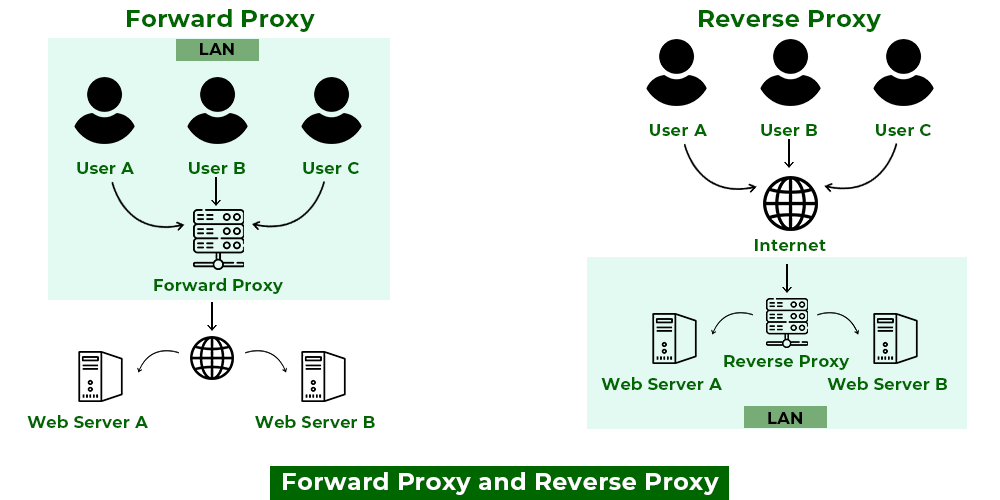
\includegraphics[width=0.6\textwidth]{graphics/Forward-Proxy-and-Reverse-Proxy.png}
    \caption{Forward versus reverse proxyserver \textcite{gfg-2023}}
    \label{fig:Forward versus reverse proxyserver} 
\end{figure}

Zoals hierboven beschreven kunnen zowel forward als reverse proxyservers worden geïnstalleerd in huidige schoolomgevingen als vervanging voor Classroom management software (CMS). Uiteraard gaan gebruikers technische kennis moeten verschaffen om deze beveiligingen aan en uit te zetten. Dit verhoogt de moeilijkheidsgraad en stressfactor bij leerkrachten tijdens schooluren. Waardoor dit niet de meest voor de hand liggende keuze wordt. Anderzijds kunnen deze wel waardevolle oplossingen bieden voor specifieke beveiligings- en beheerproblemen, maar eisen een goede implementatie en onderhoud om effectief te zijn in onderwijsinstellingen. Dit alles zorgt voor een hogere moeilijkheidsgraad en stressfactor bij leerkrachten tijdens de schooluren. 

\section{Classroom management software en proxyserver, de voor- en nadelen}
Zoals eerder besproken, zijn er twee hoofdoplossingen voor het beheren van internetgebruik tijdens de lessen: Classroom management software en proxyservers. 
Beide oplossingen hebben hun eigen voor- en nadelen, dit hangt natuurlijk af het type onderwijsinstelling, aanwezige infrastructuur en beschikbaar budget.\newline

In dit onderdeel worden de voor- en nadelen van beiden besproken en overwogen. Betrekkend tot de nadruk op activering van flexibel beheer. Aan het einde wordt er geconcludeerd welke keuze het beste is voor dit onderzoek. 
Doordat de belangrijkste vereiste het flexibel beperken en activeren van sociale media en E-commerce websites is. Dit maakt de configuratie en installatie van een proxy server een complexere taak, omdat dit moeilijker te installeren valt per leerling op een school. Daarentegen biedt het gebruik van Classroom management software een flexibele gebruiksomgeving en meerdere functies die handig kunnen zijn tijdens de lessen zoals het flexibel activeren en beperken van websites. Hieronder bevinden zich de voor- en nadelen van beide opties. \newline

\subsection{Classroom management software}
\textbf{Voordelen}
\begin{itemize}
    \item gebruiksvriendelijk: softwareontwikkelaars zorgen voor een gebruiksvriendelijke omgeving zodat leerkrachten geen extra aandacht moeten besteden aan het leerproces van het programma. 
    \item Bevatten veel functies: verwijzing naar \ref{classroom management software}
    \item Veel configuratie mogelijkheden: verwijzing naar \ref{classroom management software}
\end{itemize}
\textbf{Nadelen}
\begin{itemize}
    \item Privacy beleid volgen: verwijzing naar \ref{beveiliging en privacy CMS}
    \item Meestal betaalbaar: het merendeel van de software mogelijkheden zijn betalend of worden betalend vanaf een bepaald aantal gebruikers. Hierdoor is het niet altijd haalbaar voor onderwijsinstellingen om deze te hanteren in elke klasomgeving. 
\end{itemize}

\subsection{Proxyserver}
\textbf{Voordelen}
\begin{itemize}
    \item Goedkoop tot zelfs gratis: Doordat een standaard proxyserver makkelijk kan worden opgezet in een Linux omgeving, wordt er geen extra kosten aangerekend voor proxy services. 
    \item Veiligheid: proxies bieden een extra beschermlaag tegen kwaadaardige codes op websites, waardoor de kans op malware en virussen afneemt.
    \item Websites blacklisten: proxies bieden de mogelijkheid om specifieke websites op een blacklist te zetten. Hierdoor kan ervoor worden gekozen om sociale media of E-commerce websites te blokkeren op scholen of bedrijven. Ook wordt de browsergeschiedenis van elke gebruiker opgeslagen. Met als gevolg kunnen op elk moment de logs worden opgevraagd. 
    \item Ip-adres verbergen: een proxy verbergt je ip-adres, waardoor je online identiteit beschermt wordt tegen tracking door bedrijven. Dit vergroot de veiligheid en privacy, aangezien de activiteiten niet direct aan de gebruikers worden gelinkt. Ook gaat deze functie de gepersonaliseerde advertenties tegen.
    \autocite{Janssen2023}  
\end{itemize}
\textbf{Nadelen}
\begin{itemize}
    \item Geen volledige anonimiteit: het hanteren van proxy server biedt geen volledige privacy. Aangezien de beheerder de activiteiten kan monitoren, vooral bij gratis en open-source proxies, waarbij de controle over de verbinding onduidelijk is.
    \item Geen versleuteling: een proxyserver biedt geen absolute online veiligheid. Ook al worden uitvoeringen op het internet niet rechtstreeks naar de zender herleidt. Toch wordt deze data niet extra versleuteld waardoor websites nog altijd zicht hebben op welke persoon wat uitvoert. 
    \item IT-kennis nodig voor veranderingen: een van de grootste nadelen van een proxy server is de kennis in het vak. Voor veranderingen aan de toegang tot websites is enige IT-kennis nodig. 
    \autocite{proxyserver}
    \autocite{nordvpn}
\end{itemize}






